\documentclass[conference,a4paper]{IEEEtran}
% AMICT 2026: IEEE conference format matching TemplateAMICT2026.doc
% Companion: supplementary.tex (extended figures, protocol, code/data).
\usepackage{cite}
\usepackage{url}
\usepackage{graphicx}
\usepackage{tikz}
\usepackage{amsmath}
\usepackage{algorithm}
\usepackage{algpseudocode}
\usepackage{booktabs}
\usepackage{microtype}

\usetikzlibrary{arrows.meta,shapes.geometric}

\title{Content-Conditioned Cyclic Seam Carving for Equirectangular Panoramas}

\author{\IEEEauthorblockN{Anonymous Authors}
\IEEEauthorblockA{Affiliation withheld for double-blind review}}

\begin{document}
\maketitle

\begin{abstract}
Equirectangular (ERP) $360^\circ$ video is stored at
$4$K--$8$K for the full sphere even though a viewer sees only a
viewport, so content-aware retargeting can shrink that raster
before any viewport is extracted. On crowd panoramas we find
that cyclic routing, spherical energy, and semantic protection
help only in specific regimes: a cyclic spherical baseline
already misses most compact heads, and always-on person
protection is therefore wasted on most scenes. We propose
content-conditioned cyclic seam carving, which applies cyclic
routing and spherical energy on every image and adds semantic
energy only when a SegFormer-B0 estimate of baseline person-hit
risk is high. Experiments use stills of width at most $512$ and
$k=24$ seams. On PanoCount medium-density val+test ($n=171$) the
gate fires on $56$ images and lowers a ground-truth body-hit
proxy from $12.59\%$ to $11.04\%$ (paired $-1.55$\,pp, $95\%$ CI
$[-2.75,-0.35]$\,pp). On that subset the change is $-4.73$\,pp
($17/56$ images increase), while the remaining $115$ images keep
the spherical baseline. An oracle that sees GT columns reaches
$-35.2$\,pp on a high-risk subset, and always-on
predicted-person energy lowers instance hit from $18.68\%$ to
$5.16\%$. Sparse temporal sampling can fabricate unsupported
apparent yaw, which we report as a motion-estimation control.
Geometric and semantic constraints should be selected by content
risk.
\end{abstract}

\begin{IEEEkeywords}
equirectangular panorama, seam carving, 360-degree video, viewport,
semantic protection, cyclic routing, content-aware retargeting,
crowd panoramas
\end{IEEEkeywords}

\section{Introduction}
\label{sec:intro}

Omnidirectional video is stored as an equirectangular (ERP)
$2{:}1$ raster, often at $4$K--$8$K, even though a viewer sees
only a
viewport~\cite{hosseini2016adaptive,corbillon2017viewport,graf2017omnidirectional,qian2018flare}.
Viewport-adaptive streaming rate-allocates tiles around that
predicted field of view~\cite{corbillon2017optimal}, whereas
content-aware carving is an orthogonal lever: it removes ERP
columns before any viewport is extracted. All still-image
experiments in this paper use width at most $512$.

Seam carving removes a connected minimum-energy
path~\cite{avidan2007seam}. On an ERP that path meets a periodic
longitude, a latitude-dependent area
element~\cite{coors2018spherenet,cheng2018cubepadding}, and
persons that occupy only part of the sphere. A planar carver
that stops at the $0/W$ cut therefore produces a border seam,
unweighted energy treats polar and equatorial steps as equal,
and class-agnostic energy can cut a person on a low-energy
corridor. Those effects are strong on some panoramas and mild on
others; prior $360^\circ$
carving~\cite{tsubaki2018interrupted,choi2021distortion}
supplies the geometric contrast for this study.

Cyclic topology is a property of the domain, whereas spherical
energy and semantic energy depend on content. We propose
\emph{content-conditioned cyclic seam carving}
(Fig.~\ref{fig:method}, Algorithm~\ref{alg:ccsc}), which applies
cyclic routing and spherical energy on every image and adds
semantic energy only when predicted baseline person-hit risk is
high. A separate control tests motion estimation under sparse
sampling (Section~\ref{sec:sparse-sampling}).

An \emph{oracle} that paints GT body columns reduces high-risk
hits from $35.4\%$ to $0.2\%$ ($-35.2$\,pp). A \emph{practical}
SegFormer-B0~\cite{xie2021segformer} gate on
{ADE20K}~\cite{zhou2017ade20k} person pixels, evaluated on
PanoCount~\cite{arbi2025panocount} medium val+test ($n=171$,
$k=24$), turns $\lambda_s$ on for $56$ images and off for $115$.
GT body-hit then falls from $12.59\%$ to $11.04\%$ ($-1.55$\,pp,
$95\%$ CI $[-2.75,-0.35]$); on the ON subset the change is
$-4.73$\,pp, with $17/56$ images increasing. Always-on
predicted-person instance hit falls from $18.68\%$ to $5.16\%$.

\subsection{Contributions}
\begin{enumerate}
  \item Cyclic ERP carving with spherical energy~\eqref{eq:ep}
  and wrap-aware routing~\eqref{eq:dp}, implemented as standard
  $O(HW)$ dynamic programming. On
  {CVRG-Pano}~\cite{orhan2021semantic} the spherical term moves
  polar routing by $+0.42$\,pp.

  \item A content-conditioned gate (Algorithm~\ref{alg:ccsc})
  that sets $\lambda_s=4$ when $h_{\mathrm{pred}}\ge\tau$, with
  $\tau=0.20$ taken from the oracle high-body cutoff.

  \item A two-level evaluation: an oracle GT-column bound of
  $-35.2$\,pp, and a practical SegFormer gate of
  $12.59\%\rightarrow 11.04\%$ ($-1.55$\,pp overall;
  $-4.73$\,pp on $56$ activations, $17/56$ increasing).

  \item A motion-estimation control showing that sparse
  sampling can produce photometrically unsupported apparent yaw
  (Section~\ref{sec:sparse-sampling}).
\end{enumerate}
Extended figures, protocol, code, and remaining data are in the
supplementary material.

\section{Related Work}
\label{sec:related}

Seam carving removes a connected minimum-energy
path~\cite{avidan2007seam}. Later planar work mixed forward energy,
cropping, and scaling~\cite{rubinstein2008improved,rubinstein2009multi},
while warping~\cite{wolf2007nonhomogeneous,wang2008scale} and
shift-maps~\cite{pritch2009shiftmap} redistribute distortion
rather than delete a connected path. Class-weighted energies are
standard on planar
images~\cite{itti1998saliency,goferman2010context}. We use seam
carving because a vertical ERP path is meridian-like, and we
apply class energy only as a $\lambda_s$ term on person pixels.

Viewport-adaptive streaming rate-allocates the predicted field of
view~\cite{hosseini2016adaptive,corbillon2017viewport,corbillon2017optimal,graf2017omnidirectional,qian2018flare},
and head traces are the usual way to locate that
viewport~\cite{sitzmann2018saliencyvr,david2018headeye}. Those
systems motivate shrinking unused ERP pixels. Polar stretching is
a property of ERP
sampling~\cite{coors2018spherenet,cheng2018cubepadding}, which we
place in the seam cost through $E_p=E_g\cos\phi$. Prior
$360^\circ$ carving interrupts or warps the
cut~\cite{tsubaki2018interrupted}, weights panoramic
resizing~\cite{choi2021distortion}, or uses carving inside object
removal~\cite{macquarrie2015object}. Neural latitude-aware
rescaling~\cite{guo2023dinn360} likewise changes resolution along
a connected path. Although 360 saliency models
exist~\cite{monroy2018salnet360}, the practical gate instead
transfers ADE20K person pixels through
SegFormer-B0~\cite{xie2021segformer,zhou2017ade20k}. Video carving
couples seams across frames~\cite{rubinstein2008improved}; the
comparisons in this paper are internal: cyclic versus spherical
energy, always-on versus gated $\lambda_s$, and oracle GT columns
versus a transferred segmenter.

\section{Method}
\label{sec:method}

Fig.~\ref{fig:method} and Algorithm~\ref{alg:ccsc} summarize the
pipeline: seams are recovered by standard $O(HW)$ dynamic
programming per seam, while motion estimation is held as a
separate control (Section~\ref{sec:sparse-sampling}).

\begin{figure*}[!t]
\centering
\resizebox{\textwidth}{!}{% Vector overview of content-conditioned cyclic seam carving (no raster).
% Wide, short layout for an IEEE two-column (figure*) float.
% Color encodes later-figure convention:
% red = spherical baseline seams, magenta = person regions,
% green = gate-ON / semantic recarve.
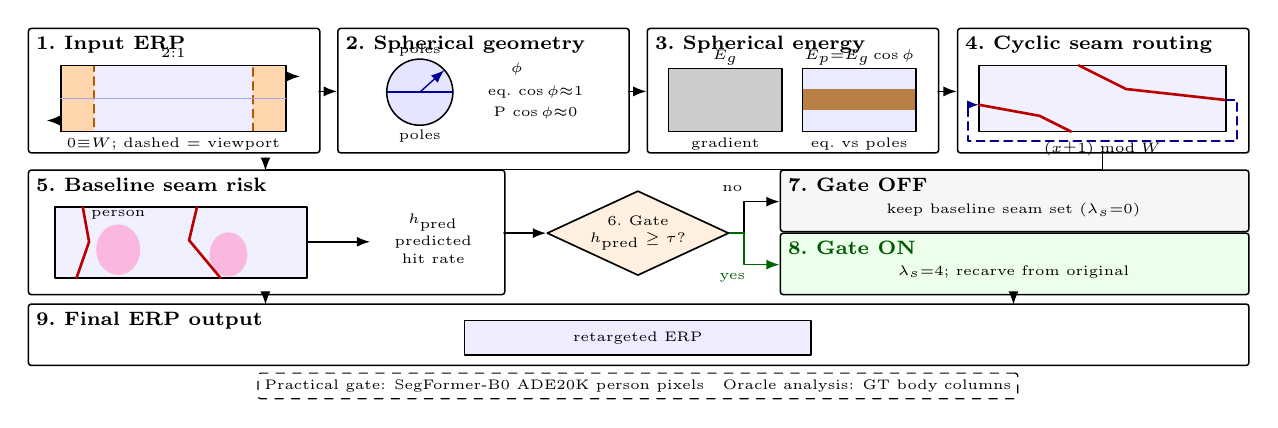
\begin{tikzpicture}[
  font=\scriptsize,
  line cap=round,
  line join=round,
  >=Latex,
  arr/.style={-{Latex[length=1.7mm]}, line width=0.6pt},
  panel/.style={
    draw,
    rounded corners=1pt,
    line width=0.55pt,
    inner sep=0pt,
    fill=white,
  },
  ptitle/.style={font=\scriptsize\bfseries, anchor=north west, inner sep=0pt},
  tiny/.style={font=\tiny},
  seam/.style={red!72!black, line width=0.95pt},
  wrap/.style={-{Latex[length=1.5mm]}, densely dashed, line width=0.55pt, blue!55!black},
]
\def\W{15.5}

% ===== Row 1: input | spherical | energy | cyclic =====
\begin{scope}[shift={(0,2.72)}]
  \node[panel, minimum width=3.70cm, minimum height=1.58cm, anchor=south west] at (0,0) {};
  \node[ptitle] at (0.10,1.50) {1.~Input ERP};
  \fill[blue!7] (0.42,0.28) rectangle (3.28,1.12);
  \fill[orange!32] (0.42,0.28) rectangle (0.84,1.12);
  \fill[orange!32] (2.86,0.28) rectangle (3.28,1.12);
  \draw[orange!70!black, densely dashed, line width=0.5pt]
    (0.42,0.28) rectangle (0.84,1.12);
  \draw[orange!70!black, densely dashed, line width=0.5pt]
    (2.86,0.28) rectangle (3.28,1.12);
  \draw[line width=0.55pt] (0.42,0.28) rectangle (3.28,1.12);
  \draw[blue!35] (0.42,0.70) -- (3.28,0.70);
  \node[tiny] at (1.85,1.28) {$2{:}1$};
  \draw[arr] (0.42,0.42) -- ++(-0.18,0);
  \draw[arr] (3.28,0.98) -- ++(0.18,0);
  \node[tiny] at (1.85,0.12) {$0{\equiv}W$; dashed = viewport};
\end{scope}

\begin{scope}[shift={(3.93,2.72)}]
  \node[panel, minimum width=3.70cm, minimum height=1.58cm, anchor=south west] at (0,0) {};
  \node[ptitle] at (0.10,1.50) {2.~Spherical geometry};
  \fill[blue!10] (1.05,0.78) circle (0.42);
  \draw[line width=0.55pt] (1.05,0.78) circle (0.42);
  \draw[blue!60!black, line width=0.5pt] (0.63,0.78) -- (1.47,0.78);
  \draw[arr, blue!60!black, line width=0.5pt] (1.05,0.78) -- ++(42:0.42);
  \node[tiny] at (1.05,1.32) {poles};
  \node[tiny] at (1.05,0.22) {poles};
  \node[tiny] at (2.28,1.08) {$\phi$};
  \node[tiny, align=left] at (2.52,0.78) {eq.\ $\cos\phi{\approx}1$};
  \node[tiny, align=left] at (2.52,0.52) {P\ $\cos\phi{\approx}0$};
\end{scope}

\begin{scope}[shift={(7.86,2.72)}]
  \node[panel, minimum width=3.70cm, minimum height=1.58cm, anchor=south west] at (0,0) {};
  \node[ptitle] at (0.10,1.50) {3.~Spherical energy};
  \fill[gray!40] (0.28,0.28) rectangle (1.72,1.08);
  \draw[line width=0.5pt] (0.28,0.28) rectangle (1.72,1.08);
  \node[tiny] at (1.00,1.22) {$E_g$};
  \fill[blue!8] (1.98,0.82) rectangle (3.42,1.08);
  \fill[orange!45!gray] (1.98,0.55) rectangle (3.42,0.82);
  \fill[blue!8] (1.98,0.28) rectangle (3.42,0.55);
  \draw[line width=0.5pt] (1.98,0.28) rectangle (3.42,1.08);
  \node[tiny] at (2.70,1.22) {$E_p{=}E_g\cos\phi$};
  \node[tiny] at (1.00,0.12) {gradient};
  \node[tiny] at (2.70,0.12) {eq.\ vs poles};
\end{scope}

\begin{scope}[shift={(11.80,2.72)}]
  \node[panel, minimum width=3.70cm, minimum height=1.58cm, anchor=south west] at (0,0) {};
  \node[ptitle] at (0.10,1.50) {4.~Cyclic seam routing};
  \fill[blue!6] (0.28,0.28) rectangle (3.42,1.12);
  \draw[line width=0.55pt] (0.28,0.28) rectangle (3.42,1.12);
  \draw[seam] (1.55,1.12) -- (2.15,0.82) -- (3.42,0.68);
  \draw[seam] (0.28,0.62) -- (1.05,0.48) -- (1.45,0.28);
  \draw[wrap]
    (3.42,0.68) -- (3.56,0.68) -- (3.56,0.16) -- (0.14,0.16) -- (0.14,0.62) -- (0.28,0.62);
  \node[tiny] at (1.85,0.06) {$(x{\pm}1)\bmod W$};
\end{scope}

\draw[arr] (3.70,3.51) -- (3.93,3.51);
\draw[arr] (7.63,3.51) -- (7.86,3.51);
\draw[arr] (11.56,3.51) -- (11.80,3.51);

% ===== Row 2: risk | gate | OFF/ON =====
\begin{scope}[shift={(0,0.92)}]
  \node[panel, minimum width=6.05cm, minimum height=1.58cm, anchor=south west] at (0,0) {};
  \node[ptitle] at (0.10,1.50) {5.~Baseline seam risk};
  \fill[blue!6] (0.35,0.22) rectangle (3.55,1.12);
  \draw[line width=0.55pt] (0.35,0.22) rectangle (3.55,1.12);
  \fill[magenta!28] (1.15,0.58) ellipse (0.28 and 0.32);
  \fill[magenta!28] (2.55,0.52) ellipse (0.24 and 0.28);
  \node[tiny] at (1.15,1.02) {person};
  \draw[seam] (0.70,1.12) -- (0.78,0.68) -- (0.62,0.22);
  \draw[seam] (2.15,1.12) -- (2.05,0.70) -- (2.45,0.22);
  \draw[arr] (3.55,0.68) -- (4.35,0.68);
  \node[tiny, align=center] at (5.15,0.92) {$h_{\mathrm{pred}}$};
  \node[tiny, align=center] at (5.15,0.68) {predicted};
  \node[tiny, align=center] at (5.15,0.46) {hit rate};
\end{scope}

\node[draw, diamond, aspect=2.15, inner sep=0.8pt, line width=0.6pt,
  fill=orange!12, font=\tiny, align=center]
  (gate) at (7.75,1.71) {6.~Gate\\$h_{\mathrm{pred}}\ge\tau$?};

\begin{scope}[shift={(9.55,1.72)}]
  \node[panel, fill=gray!7, minimum width=5.95cm, minimum height=0.78cm, anchor=south west] at (0,0) {};
  \node[ptitle] at (0.10,0.70) {7.~Gate OFF};
  \node[tiny] at (2.97,0.28) {keep baseline seam set ($\lambda_s{=}0$)};
\end{scope}

\begin{scope}[shift={(9.55,0.92)}]
  \node[panel, fill=green!8, minimum width=5.95cm, minimum height=0.78cm, anchor=south west] at (0,0) {};
  \node[ptitle, green!35!black] at (0.10,0.70) {8.~Gate ON};
  \node[tiny, align=center] at (2.97,0.30) {$\lambda_s{=}4$; recarve from original};
\end{scope}

\draw[arr] (13.65,2.72) -- (13.65,2.52) -| (3.02,2.50);
\draw[arr] (6.05,1.71) -- (gate.west);
\draw[arr] (gate.east) -- ++(0.18,0) |- (9.55,2.11);
\node[tiny] at (8.95,2.28) {no};
\draw[arr, green!40!black] (gate.east) -- ++(0.18,0) |- (9.55,1.31);
\node[tiny, green!35!black] at (8.95,1.14) {yes};

% ===== Row 3: final output =====
\begin{scope}[shift={(0,0.02)}]
  \node[panel, minimum width=\W cm, minimum height=0.78cm, anchor=south west] at (0,0) {};
  \node[ptitle] at (0.10,0.70) {9.~Final ERP output};
  \fill[blue!7] (5.55,0.14) rectangle (9.95,0.58);
  \draw[line width=0.55pt] (5.55,0.14) rectangle (9.95,0.58);
  \node[tiny] at (7.75,0.36) {retargeted ERP};
\end{scope}

\draw[arr] (12.52,0.92) -- (12.52,0.80);
\draw[arr] (3.02,0.92) -- (3.02,0.80);

\node[draw, dashed, rounded corners=1pt, line width=0.45pt, inner sep=2.4pt,
  align=left, font=\tiny, anchor=north] at (7.75,-0.06) {%
  Practical gate: SegFormer-B0 ADE20K person pixels\quad
  Oracle analysis: GT body columns};

\end{tikzpicture}
}
\caption{Overview of content-conditioned cyclic seam carving.
Panel~1 marks a schematic viewport whose ERP support wraps the
$0/W$ cut (dashed orange). Cyclic seam routing and spherical
energy run on every image. The gate inspects predicted-person
instances on the spherical baseline and, if
$h_{\mathrm{pred}}\ge\tau$, recomputes seams with semantic
energy; otherwise the baseline seam set is kept. Red: spherical
baseline. Magenta: person regions. Green: gate-ON branch.}
\label{fig:method}
\end{figure*}

\subsection{Energy}
\label{sec:energy}

Let $I$ be an RGB ERP of size $H\times W$, with column $x$ as
longitude and row $y$ as latitude, so that latitude at row $y$ is
\begin{equation}
\label{eq:phi}
\phi(y)=\Bigl(\frac{y}{H-1}-\tfrac12\Bigr)\pi.
\end{equation}
Gradient energy $E_g$ is computed with circular padding in $x$,
and spherical energy is
\begin{equation}
\label{eq:ep}
E_p=E_g\cos\phi,
\end{equation}
where $\phi$ is given by~\eqref{eq:phi}. A semantic map $E_s$
assigns a higher cost to protected pixels (persons) than to
background. After independent min-max normalization of each term
to $[0,1]$, the combined energy is
\begin{equation}
\label{eq:combine}
E=\lambda_g\tilde E_g+\lambda_p\tilde E_p+\lambda_s\tilde E_s,
\end{equation}
with $\lambda_g=\lambda_p=1$ throughout. Configuration (b) uses
$\lambda_s=0$ and configuration (c) uses $\lambda_s=4$; the source
of $E_s$ is experiment-specific (GT head disks, GT body columns,
or predicted person pixels).

For GT heads, the latitude-aware $2^\circ$ radius is
\begin{equation}
\label{eq:rphi}
r(\phi)=\frac{r_{\mathrm{eq}}}{\max\bigl(|\cos\phi|,\cos 75^\circ\bigr)},
\quad
r_{\mathrm{eq}}=W\cdot\frac{2^\circ}{360}.
\end{equation}
Oracle body columns extend $12^\circ$ of latitude down from each
head, with half-width $2.5\,r(\phi)$.

\subsection{Cyclic Seam Routing}
\label{sec:cyclic}

A vertical seam $S\in\{0,\ldots,W-1\}^H$ is an eight-connected
path with one column per row. Cyclic seam routing uses the
wrap-around neighbors $P(x)=\{x-1,x,x+1\}\bmod W$, so the
forward recurrence is
\begin{equation}
\label{eq:dp}
M(y,x)=E(y,x)+\min_{x'\in P(x)} M(y-1,x').
\end{equation}
The seam is recovered by backward argmin, and a width reduction
of $k$ pixels repeats this $k$ times with energy recomputed after
each removal. Complexity is $O(kHW)$: wrap-around changes the
neighbor set but not the asymptotic cost.

Because a viewport can wrap columns $0$ and $W-1$
(Fig.~\ref{fig:method}), cyclic neighbors make the seam a closed
meridian under that yaw. Reported scores are polar routing share
and person-hit on the full ERP.

\subsection{Content-Conditioned Gate}
\label{sec:gate}

Cyclic seam routing and spherical energy~\eqref{eq:ep} run on
every image; semantic energy is applied only when needed. Let
$h_{\mathrm{pred}}$ be the predicted-person instance hit rate of
the first $k$ original-width (b) seams. The gate is
\begin{equation}
\label{eq:gate}
\lambda_s=
\begin{cases}
4 & \text{if }h_{\mathrm{pred}}\ge\tau,\\
0 & \text{otherwise,}
\end{cases}
\end{equation}
with $\tau=0.20$ and $k=24$ in the practical experiment, copying
the oracle high-body cutoff onto $h_{\mathrm{pred}}$. If the gate
is on, seams are recomputed from the original image
under~\eqref{eq:combine} with $\lambda_s=4$; if it is off, the
(b) seam set is kept. The oracle analysis uses the same
threshold form on GT body-column hits (Section~\ref{sec:setup}),
and Algorithm~\ref{alg:ccsc} is the practical procedure.

\begin{algorithm}[H]
\caption{Content-conditioned cyclic seam carving (practical gate)}
\label{alg:ccsc}
\begin{algorithmic}[1]
\Require ERP image $I$, seam count $k$, threshold $\tau$
\Ensure seam set $S$
\State Compute $E_g$ and $E_p=E_g\cos\phi$ as in \eqref{eq:ep}
\State $S^{(b)}\gets$ cyclic carve of $I$ with \eqref{eq:combine}, $\lambda_s=0$
\State $h_{\mathrm{pred}}\gets$ predicted-person instance hit rate of $S^{(b)}$
\If{$h_{\mathrm{pred}}\ge\tau$}
  \State $S\gets$ cyclic carve of $I$ with \eqref{eq:combine}, $\lambda_s=4$ on the predicted person map
\Else
  \State $S\gets S^{(b)}$
\EndIf
\end{algorithmic}
\end{algorithm}

\section{Experimental Setup}
\label{sec:setup}

All still-image carves use cyclic seam routing~\eqref{eq:dp},
width at most $512$, and, unless noted, $k=24$ with energy
recomputed after each removal. Extended metric definitions and
the SegFormer instance protocol are in the supplementary
material.

\textbf{Datasets.}
{CVRG-Pano}~\cite{orhan2021semantic} official val+test ($n=120$)
is the spherical-energy split (Section~\ref{sec:spherical}).
PanoCount~\cite{arbi2025panocount} stills and head-point JSON
cover official val+test ($n=313$), with density bins following
the dataset: sparse $0$--$49$ ($n=72$), medium $50$--$199$
($n=171$; the claim bin), and dense $200+$ ($n=70$). Clips ERP2,
ERP4, and ERP5 are the motion-estimation control
(Section~\ref{sec:sparse-sampling}).

\textbf{Configurations.}
On PanoCount, (b) is the spherical baseline
($\lambda_g=\lambda_p=1$, $\lambda_s=0$) and (c) is always-on
semantic energy ($\lambda_s=4$). Both use cyclic routing and are
carved independently from the original image; the
content-conditioned method selects (c) if~\eqref{eq:gate} fires
and (b) otherwise. Semantic maps (GT $2^\circ$ disks, GT body
columns, or predicted person pixels) are stated with each result.
C1 on CVRG-Pano holds cyclic routing and $\lambda_s=0$ and
changes only unweighted Sobel versus $E_p=E_g\cos\phi$.

\textbf{Metrics.}
Polar occupancy and routing share use the top and bottom $15\%$
of rows, so occupancy is fixed by band height. Head-hit uses
cyclic $|x-x_{\mathrm{head}}|\le r(\phi)$ on the head row, and
body-hit uses a constructed $12^\circ$ meridian strip of
half-width $2.5\,r(\phi)$. Predicted-person instance hit scores
SegFormer components. Temporal validation uses equatorial phase
correlation~\cite{reddy1996fft} and post-warp photometry.

\textbf{Practical gate.}
SegFormer-B0~\cite{xie2021segformer} trained on
{ADE20K}~\cite{zhou2017ade20k} supplies a person map, with
instances taken as planar eight-connected components on the
$H\times W$ grid. The gate~\eqref{eq:gate} is per-image:
$\lambda_s=4$ iff $h_{\mathrm{pred}}\ge\tau=0.20$. GT body-hit is
an external score; the gate observes predicted instances.

\textbf{Statistics.}
For all-medium gated GT body-hit, $\delta_i$ is gated minus (b)
on panorama $i$. The mean is $\bar{\delta}=(1/n)\sum_i\delta_i$
with $n=171$, and the $95\%$ interval is the paired
normal-approximation CI
\begin{equation}
\label{eq:ci}
\bar{\delta}\,\pm\,1.96\cdot\mathrm{std}(\delta)/\sqrt{n}.
\end{equation}
Many $\delta_i$ are exactly zero (all gate-off images), so the
mean mixes a point mass at zero with a minority of nonzero
changes.

\section{Results}
\label{sec:results}

Cyclic seam routing is held fixed; what varies is spherical
energy, always-on semantic energy, or the content-conditioned
gate.

\subsection{RQ1: How does ERP geometry affect seam routing?}
\label{sec:spherical}

Cyclic routing sets the legal neighbors
($\{x-1,x,x+1\}\bmod W$) as in~\eqref{eq:dp}, while spherical
energy~\eqref{eq:ep} rescales the cost of those neighbors. On
CVRG-Pano val+test ($n=120$), both sides use cyclic DP, $k=24$,
$W\le 512$, and $\lambda_s=0$, so only Sobel versus
$E_p=E_g\cos\phi$ changes. Polar occupancy is fixed by the
$15\%$ caps ($0.297$); the spherical signal is polar routing
share.

\begin{table}[t]
\centering
\caption{Polar routing on CVRG-Pano val+test ($n=120$, $k=24$).
Both rows use cyclic routing; only~\eqref{eq:ep} changes.
Values are mean${}\pm{}$std.}
\label{tab:spherical}
\small
\setlength{\tabcolsep}{3pt}
\resizebox{\columnwidth}{!}{%
\begin{tabular}{lccc}
\toprule
Method & Occupancy & Routing share & Mean polar $|\Delta x|$ \\
\midrule
Plain Sobel, cyclic & $0.297\pm 0$ & $0.301\pm 0.015$ & $0.766$ \\
Sobel $\times\cos\phi$, cyclic & $0.297\pm 0$ & $0.306\pm 0.014$ & $0.772$ \\
Paired $\Delta$ & $0.000$ & $+0.0042\pm 0.007$ & $+0.007$ \\
\bottomrule
\end{tabular}}
\end{table}

Occupancy is bit-identical, while routing rises from $0.301$ to
$0.306$ ($\Delta=+0.42$\,pp; $89/120$ up, $31$ down) and mean
polar step moves $+0.007$\,px. Only $23/120$ images move by more
than $+1$\,pp, and the unweighted polar/equator Sobel ratio is
uncorrelated with $\Delta$ (Spearman $\rho=-0.01$;
Fig.~\ref{fig:c1-scatter}). On this corpus the spherical term is
therefore a small routing shift.

\begin{figure}[t]
  \centering
  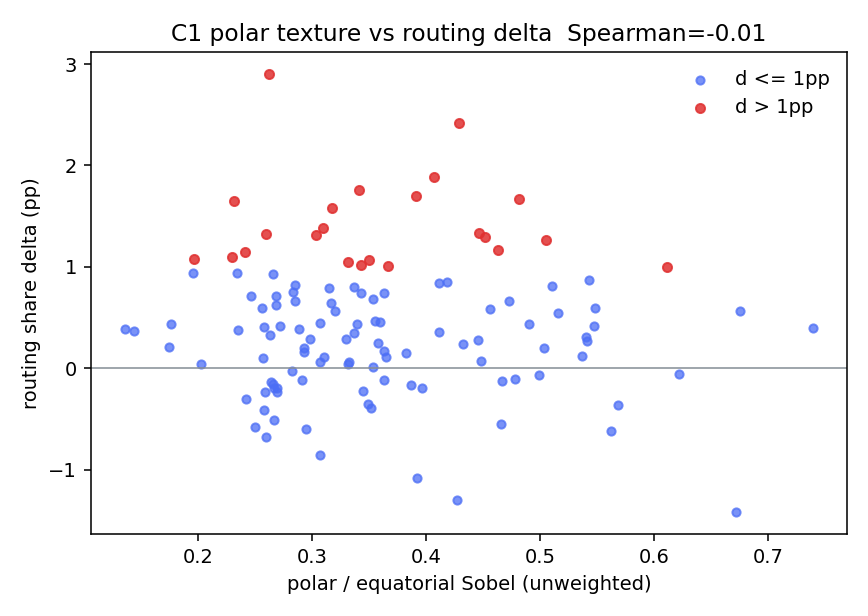
\includegraphics[width=0.82\linewidth]{figures/fig_c1_polar_scatter.png}
  \caption{Unweighted polar/equator Sobel ratio versus polar
  routing $\Delta$ on CVRG-Pano ($n=120$). Spearman
  $\rho=-0.01$. Red points: $\Delta>+1$\,pp.}
  \label{fig:c1-scatter}
\end{figure}

\subsection{RQ2: When does semantic protection matter?}
\label{sec:head-disks}

Always-on protection of $2^\circ$ GT head disks~\eqref{eq:rphi}
on PanoCount val+test, $k=24$, yields a limited aggregate
reduction (Table~\ref{tab:head-disks}): medium falls from
$4.3\%$ to $0.1\%$ ($\Delta=-4.18$\,pp), with (c)$<$(b) on
$82/171$ images. The pre-specified support bar was at least
$5$\,pp and a majority of images with (c)$<$(b); medium misses
both. Medium (b) already hits only $4.3\%$ of heads, so
$-4.18$\,pp uses essentially that range, while (c) improves on
(b) at $k=24$ on all $313$ images. $k=48$ would give $-8.73$\,pp
on medium. Scoring the same (b) seams against body columns
places medium at $12.6\%$. Fig.~\ref{fig:head-max}(a)--(b) shows
the largest medium head-hit reduction; $87/171$ medium frames are
$0\to 0$.

\begin{table}[!b]
\centering
\caption{Always-on $2^\circ$ GT head-disk protection, PanoCount
val+test, $k=24$. (b)/(c) are head-hit rates.}
\label{tab:head-disks}
\setlength{\tabcolsep}{3.5pt}
\small
\begin{tabular}{lrrrrrr}
\toprule
Bin & $N$ & (b) & (c) & $\Delta$ (pp) & (c)$<$(b) & Eq.\ cover \\
\midrule
Sparse $0$--$49$ & $72$ & $4.5\%$ & $0.1\%$ & $-4.39$ & $26/72$ & $0.8\%$ \\
Medium $50$--$199$ & $171$ & $4.3\%$ & $0.1\%$ & $-4.18$ & $82/171$ & $2.2\%$ \\
Dense $200+$ & $70$ & $3.7\%$ & $0.0\%$ & $-3.64$ & $31/70$ & $5.3\%$ \\
\bottomrule
\end{tabular}
\end{table}

\begin{figure*}[t]
  \centering
  \begin{minipage}[t]{0.495\linewidth}
    \centering
    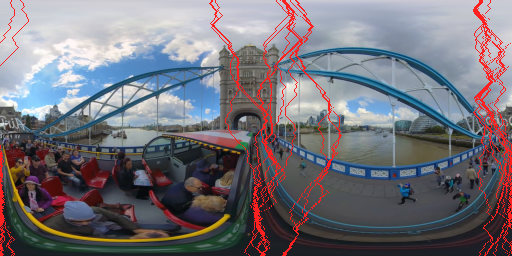
\includegraphics[height=3.15cm,keepaspectratio]{figures/fig_head_max_b.png}\\
    {\scriptsize (a) Head disks, spherical (b)}
  \end{minipage}\hfill
  \begin{minipage}[t]{0.495\linewidth}
    \centering
    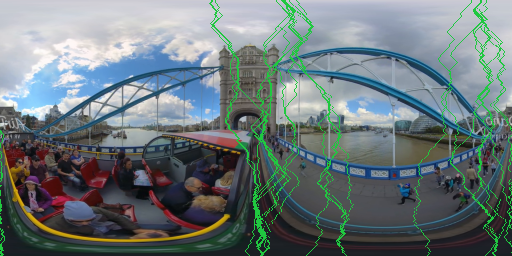
\includegraphics[height=3.15cm,keepaspectratio]{figures/fig_head_max_c.png}\\
    {\scriptsize (b) Head disks, $2^\circ$ energy (c)}
  \end{minipage}\\[3pt]
  \begin{minipage}[t]{0.495\linewidth}
    \centering
    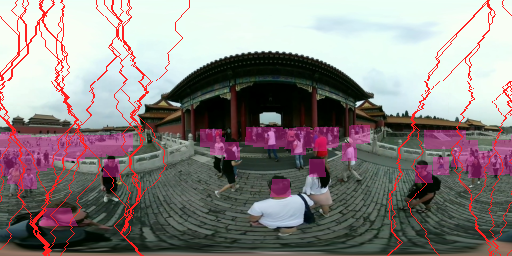
\includegraphics[height=3.15cm,keepaspectratio]{figures/fig_body_seams_b.png}\\
    {\scriptsize (c) Body columns, spherical (b)}
  \end{minipage}\hfill
  \begin{minipage}[t]{0.495\linewidth}
    \centering
    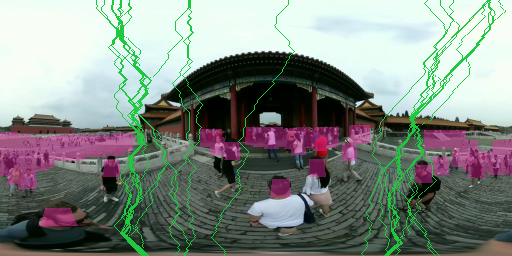
\includegraphics[height=3.15cm,keepaspectratio]{figures/fig_body_seams_c.png}\\
    {\scriptsize (d) Body columns, GT energy (c)}
  \end{minipage}
  \caption{Largest-change ERP examples at $k=24$. (a)--(b)~PanoCount
  medium, always-on $2^\circ$ GT head-disk energy. Red: spherical
  baseline. Green: (c). (c)--(d)~Largest oracle high-body case.
  Magenta: constructed GT body columns. Red: spherical baseline.
  Green: always-on $\lambda_s=4$.}
  \label{fig:head-max}
  \label{fig:body-seams}
\end{figure*}

\subsection{Content-Conditioned Semantic Protection}
\label{sec:body-boundary}

Body-column energy, $k=24$, paints GT heads as meridian strips
$12^\circ$ down, half-width $2.5\times$ the $2^\circ$ radius.
High-body is locked from (b) before (c) as the medium images
whose spherical seams already hit at least $20\%$ of those
columns ($n=49$), with complement $n=122$.
Table~\ref{tab:conditioned}(A) is an \emph{oracle}: energy and
split both see GT columns.

On oracle high-body, (c) drives GT body-hits from $35.4\%$ to
$0.2\%$ ($-35.2$\,pp) on every image. On the complement, (b)
already hits $3.4\%$, so (c) uses that ceiling ($-3.4$\,pp).
Fig.~\ref{fig:body-seams}(c)--(d) shows the largest oracle
high-body example.

\subsubsection{Practical gate}
The practical gate uses SegFormer-B0 ADE20K person instances
(Section~\ref{sec:setup}), $\tau=0.20$, and $k=24$
(Algorithm~\ref{alg:ccsc}). On PanoCount medium ($n=171$) it
turns $\lambda_s$ on for $56$ images and off for $115$
(Table~\ref{tab:conditioned}(A)), and mean GT body-hit falls from
$12.59\%$ to $11.04\%$ ($\Delta=-1.55$\,pp, $95\%$ CI
$[-2.75,-0.35]$). On the $56$ ON images the same metric changes
by $-4.73$\,pp (CI $[-8.28,-1.19]$): $34/56$ down, $5/56$ tied,
and $17/56$ up (Fig.~\ref{fig:qual}d). Gate-off $\Delta=0$ by
construction. The ON set overlaps oracle high-body on $30/49$
and misses $19/49$; it also fires on $26$ images outside that
subset. Always-on predicted-person instance hit falls from
$18.68\%$ to $5.16\%$ (Table~\ref{tab:conditioned}(B)). Extended
notes on the selection rule are in the supplementary material.

\subsection{Temporal Validation}
\label{sec:sparse-sampling}

Equatorial phase correlation~\cite{reddy1996fft} on one ERP2
frame ($I_t$, source $1626$, $W=512$) recovers a known cyclic
yaw exactly with zero post-warp residual, reports pan $0$ on the
next video frame ($\Delta t=0.03$\,s), and at a $7.74$\,s
linspace gap reports $253$\,px on the worst pair while the
residual ratio remains $0.95$. Sparse sampling can therefore
fabricate unsupported apparent yaw. Consecutive-frame windows of
ERP2, ERP4, and ERP5 in this corpus agree near zero;
Fig.~\ref{fig:c3-control} shows the three-condition control.

\begin{figure}[!b]
  \centering
  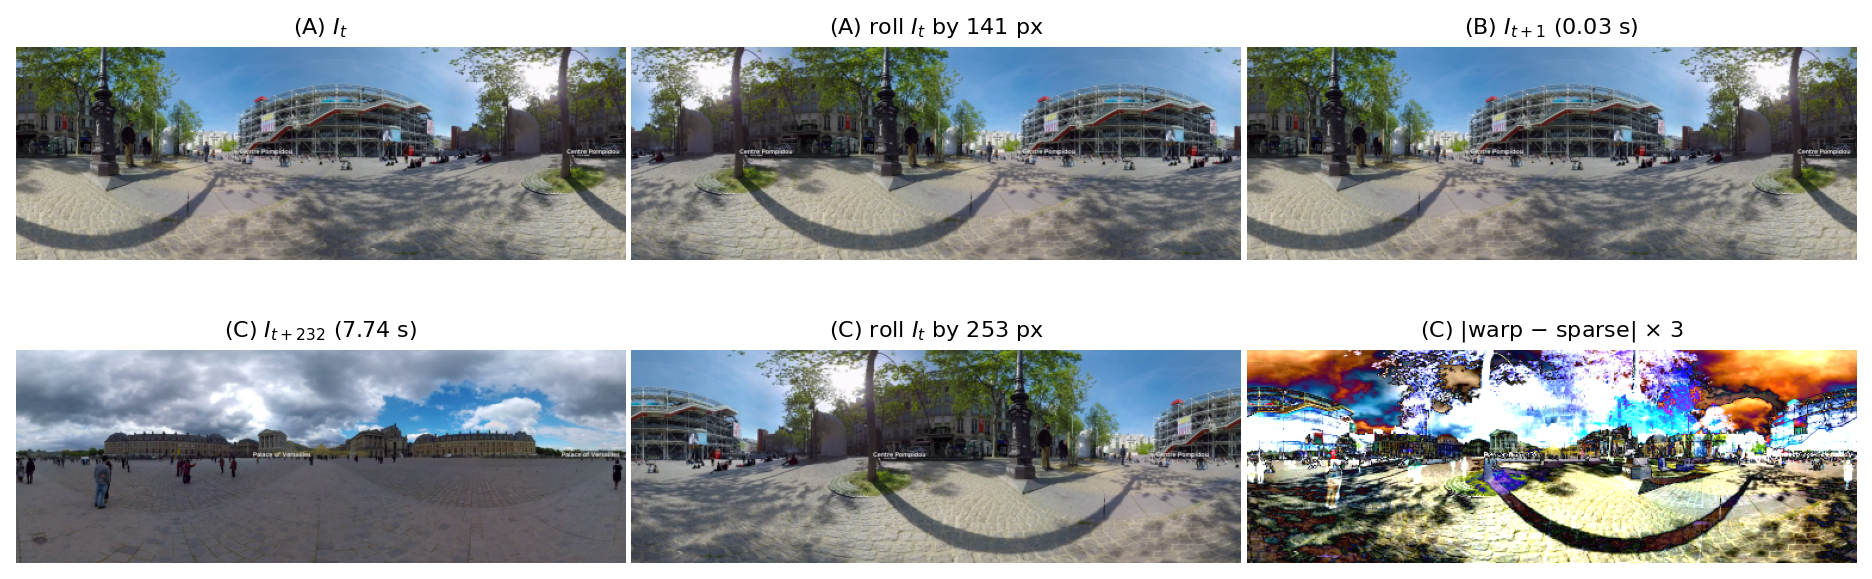
\includegraphics[width=\columnwidth]{figures/fig_c3_control.png}
  \caption{Same ERP frame $I_t$ (clip ERP2, source $1626$),
  equatorial band. (A)~A known $141$\,px cyclic roll is recovered
  exactly. (B)~The next video frame is already aligned (pan~$0$).
  (C)~At $7.74$\,s the estimator reports $253$\,px, but rolling
  $I_t$ by that amount leaves residual ratio $0.95$. Photometric
  residual is the validation criterion.}
  \label{fig:c3-control}
\end{figure}

\subsection{Qualitative Results}
\label{sec:qualitative}

Fig.~\ref{fig:qual} shows four medium PanoCount cases, with
magenta SegFormer predicted person pixels, red spherical (b)
seams, and green gated output. Stem $166$ is gate OFF with GT
$0$; stem $242$ is gate OFF with residual GT body-hit $16.9\%$;
stem $800$ is gate ON with GT down ($26.7\%\rightarrow 15.5\%$),
one of $34/56$; and stem $915$ is gate ON with GT up
($11.7\%\rightarrow 22.3\%$), one of $17/56$.

\begin{table*}[t]
\centering
\caption{Oracle versus practical content-conditioned protection
on PanoCount medium, $k=24$. (A)~GT body-hit (\% of constructed
GT persons). (B)~predicted-person instance hit (\% of SegFormer
components). $\Delta$ in percentage points. CI is~\eqref{eq:ci}.
A dash (---) marks rows where a CI was omitted. Panels are different
metrics.}
\label{tab:conditioned}
\label{tab:body-boundary}
\label{tab:practical-gate}
\setlength{\tabcolsep}{2.8pt}
\scriptsize
\begin{tabular}{l r r c c c c}
\toprule
\multicolumn{7}{l}{\textbf{(A)} Evaluation: GT body-hit} \\
\midrule
Method & $N$ & Gate ON & Before & After & $\Delta$ (pp) & $95\%$ CI \\
\midrule
Oracle high-body$^{\mathrm{a}}$ & $49$ & $49$ & $35.4\%$ & $0.2\%$ & $-35.2$ & --- \\
Oracle complement$^{\mathrm{a}}$ & $122$ & $0$ & $3.4\%$ & $0.0\%$ & $-3.4$ & --- \\
Practical predicted gate (all medium)$^{\mathrm{b}}$ & $171$ & $56$ & $12.59\%$ & $11.04\%$ & $-1.55$ & $[-2.75,-0.35]$ \\
Practical gate ON subset$^{\mathrm{b}}$ & $56$ & $56$ & $23.64\%$ & $18.90\%$ & $-4.73$ & $[-8.28,-1.19]$ \\
Practical gate OFF subset$^{\mathrm{b}}$ & $115$ & $0$ & $7.21\%$ & $7.21\%$ & $0$ & --- \\
\midrule
\multicolumn{7}{l}{\textbf{(B)} Evaluation: predicted-person instance-hit$^{\mathrm{b}}$} \\
\midrule
Always-on predicted-person$^{\mathrm{c}}$ & $171$ & $171$ & $18.68\%$ & $5.16\%$ & $-13.52$ & --- \\
\bottomrule
\end{tabular}

\vspace{4pt}
\begin{minipage}{\linewidth}
\raggedright\scriptsize
$^{\mathrm{a}}$GT-derived columns. Oracle After is always-on (c)
on the subset.\\
$^{\mathrm{b}}$SegFormer-B0 ADE20K person components. Practical
After is gated except in panel~(B).\\
$^{\mathrm{c}}$Always-on predicted-person instance hit.
\end{minipage}
\end{table*}

\begin{figure*}[t]
  \centering
  \begin{minipage}[t]{0.495\linewidth}
    \centering
    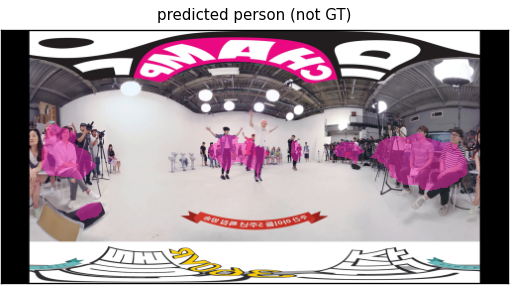
\includegraphics[width=0.325\linewidth]{figures/fig_qual_166_pred.png}%
    \hfill
    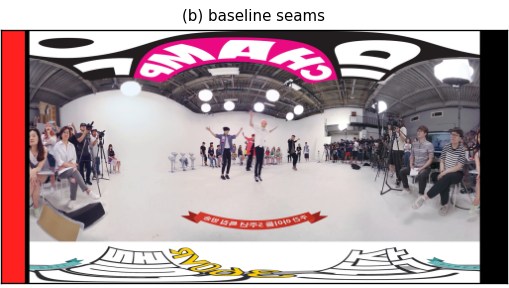
\includegraphics[width=0.325\linewidth]{figures/fig_qual_166_b.png}%
    \hfill
    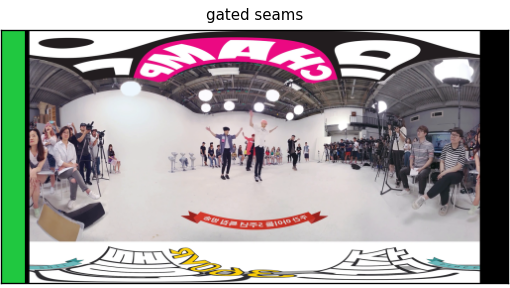
\includegraphics[width=0.325\linewidth]{figures/fig_qual_166_g.png}\\
    {\scriptsize (a) Stem $166$, OFF.
      $h_{\mathrm{pred}}=0$, GT $0\rightarrow 0$.}
  \end{minipage}\hfill
  \begin{minipage}[t]{0.495\linewidth}
    \centering
    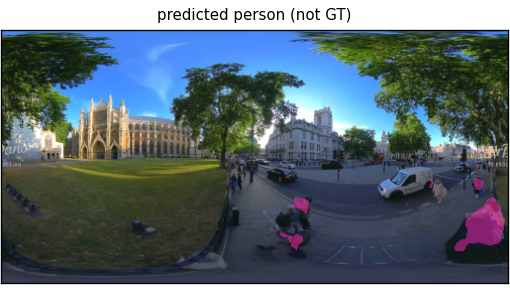
\includegraphics[width=0.325\linewidth]{figures/fig_qual_242_pred.png}%
    \hfill
    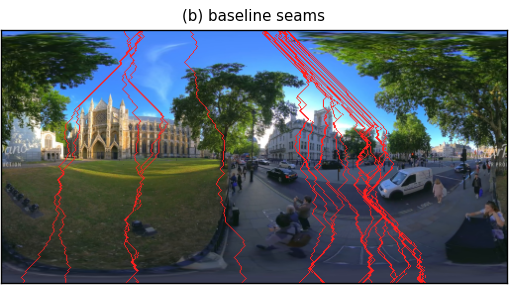
\includegraphics[width=0.325\linewidth]{figures/fig_qual_242_b.png}%
    \hfill
    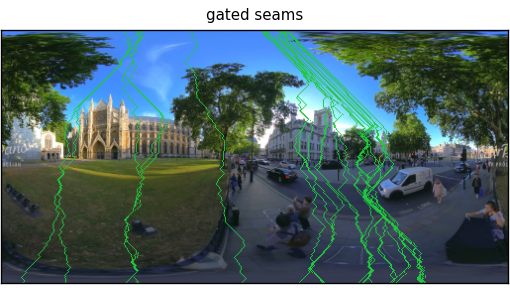
\includegraphics[width=0.325\linewidth]{figures/fig_qual_242_g.png}\\
    {\scriptsize (b) Stem $242$, OFF.
      $h_{\mathrm{pred}}=0$, GT remains $16.9\%$.}
  \end{minipage}\\[5pt]
  \begin{minipage}[t]{0.495\linewidth}
    \centering
    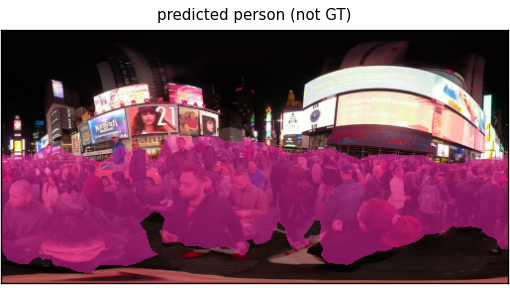
\includegraphics[width=0.325\linewidth]{figures/fig_qual_800_pred.png}%
    \hfill
    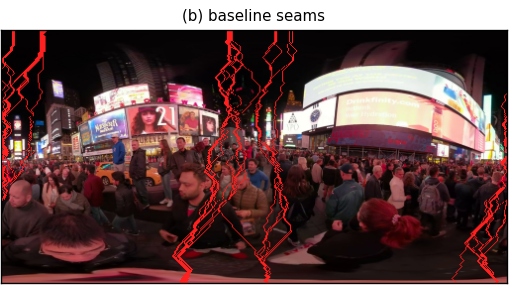
\includegraphics[width=0.325\linewidth]{figures/fig_qual_800_b.png}%
    \hfill
    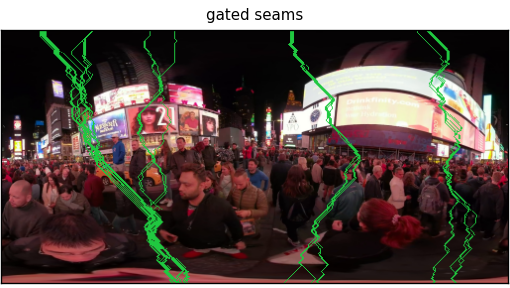
\includegraphics[width=0.325\linewidth]{figures/fig_qual_800_g.png}\\
    {\scriptsize (c) Stem $800$, ON.
      GT $26.7\%\rightarrow 15.5\%$.}
  \end{minipage}\hfill
  \begin{minipage}[t]{0.495\linewidth}
    \centering
    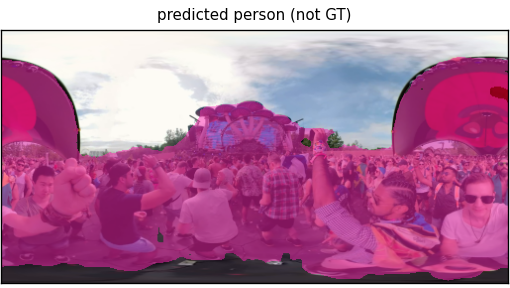
\includegraphics[width=0.325\linewidth]{figures/fig_qual_915_pred.png}%
    \hfill
    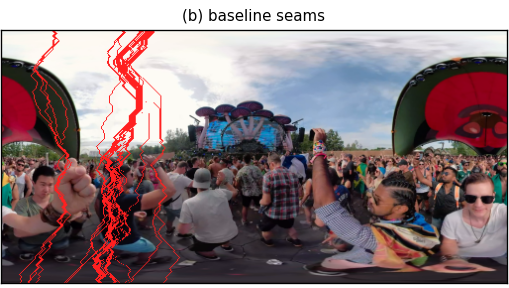
\includegraphics[width=0.325\linewidth]{figures/fig_qual_915_b.png}%
    \hfill
    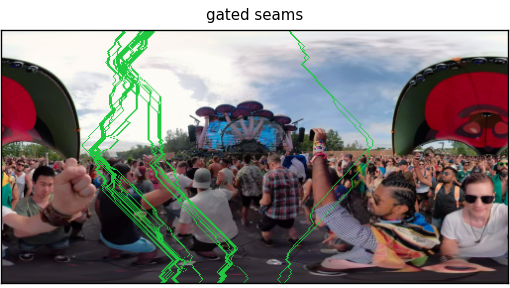
\includegraphics[width=0.325\linewidth]{figures/fig_qual_915_g.png}\\
    {\scriptsize (d) Stem $915$, ON.
      GT $11.7\%\rightarrow 22.3\%$.}
  \end{minipage}
  \caption{Practical-gate cases on PanoCount medium. In each
  triplet, left is the predicted-person overlay, middle is
  spherical (b) seams, right is gated seams. Magenta:
  SegFormer-B0 ADE20K person pixels. Red: (b). Green: gated
  output. GT body-hit is the evaluation score;
  $h_{\mathrm{pred}}$ is the gate statistic.}
  \label{fig:qual}
\end{figure*}

\section{Discussion}
\label{sec:discussion}

Cyclic routing and spherical energy do different jobs.
Routing~\eqref{eq:dp} is the legal neighbor set, fixed in every
carve so that the path is a wrap-aware meridian, whereas
spherical energy~\eqref{eq:ep} rescales step cost. On CVRG-Pano,
with routing already cyclic, $E_p=E_g\cos\phi$ moves polar
routing by $+0.42$\,pp (Table~\ref{tab:spherical}), and polar
texture is uncorrelated with that $\Delta$ ($\rho=-0.01$;
Fig.~\ref{fig:c1-scatter}). Geometry in the cost is required for
a spherical formulation; on this outdoor set the routing change
is small.

The intended consumer of a carved ERP is a
viewport~\cite{corbillon2017viewport,qian2018flare}. Cyclic
routing remains legal when yaw wraps columns $0$ and $W-1$, and
person protection concerns content that a viewport should still
contain if it looks at
people~\cite{sitzmann2018saliencyvr,david2018headeye}. The tables
report polar routing share and person-hit on the ERP.

Semantic energy is regime-dependent. Medium GT $2^\circ$ disks
are already missed by spherical seams ($4.3\%$ hit), so
always-on head-scale protection has little remaining work
(Table~\ref{tab:head-disks}). At body scale, oracle GT columns
give $-35.2$\,pp where the baseline already cuts people and
$-3.4$\,pp on the complement (Table~\ref{tab:conditioned}(A)).
The practical gate has the same shape at a smaller scale:
$-1.55$\,pp on all medium, $-4.73$\,pp on $56$ activations
($17/56$ increasing on GT), and $0$ on $115$ OFF images. The
oracle bound, the gated GT body-hit, and the always-on
predicted-person instance hit ($5.16\%$) are three different
quantities.

Phase correlation is exact on a known yaw and reports pan $0$ on
adjacent frames, whereas sparse linspace sampling can fabricate
unsupported apparent yaw (Section~\ref{sec:sparse-sampling});
photometric residual is the validation criterion.

\section{Limitations}
\label{sec:limitations}

The practical gate transfers SegFormer-B0~\cite{xie2021segformer}
trained on perspective {ADE20K}~\cite{zhou2017ade20k}. Predicted
instances are planar eight-connected components on the
$H\times W$ grid, and $\tau=0.20$ copies the oracle high-body
cutoff, so gate ON can raise GT body-hit ($17/56$) and can miss
oracle high-body images ($19/49$). The SegFormer run followed
the oracle analysis. The $95\%$ CI~\eqref{eq:ci} describes the
paired mean on $n=171$, including a point mass at zero on
gate-off images.

Stills use $W\le 512$ and primary $k=24$; GT body-hit is a
constructed $12^\circ$ column, and the temporal tests bound a
motion estimator rather than a retargeted video. Natural next
measurements include an ERP-aware segmenter, a calibrated gate,
viewport crops or HMD renders, and a comparison to Tsubaki and
Sasaki, Choi \emph{et al.}, Guo
\emph{et al.}~\cite{tsubaki2018interrupted,choi2021distortion,guo2023dinn360},
and planar crop/warp
retargeting~\cite{wang2008scale,pritch2009shiftmap,rubinstein2010comparative}.

\section{Conclusion}
\label{sec:conclusion}

ERP seam carving should apply geometric and semantic constraints
according to topology, latitude, and content risk. Cyclic seam
routing makes a legal meridian-like path, while spherical energy
is a latitude cost whose routing effect on outdoor poles is
small once that topology is in place. Semantic energy matters
where baseline seams already cut people, and has little
remaining work where they already miss.

Semantic protection on ERP is therefore regime-dependent, and a
baseline-risk rule can invoke it on a minority of images
(Fig.~\ref{fig:method}, Algorithm~\ref{alg:ccsc}). An oracle that
paints GT body columns bounds the high-risk regime at
$-35.2$\,pp. A practical SegFormer-B0~\cite{xie2021segformer}
gate, trained on {ADE20K}~\cite{zhou2017ade20k} and evaluated on
PanoCount~\cite{arbi2025panocount} medium ($n=171$, $k=24$,
$W\le 512$), reduces constructed body-hit from $12.59\%$ to
$11.04\%$ ($-1.55$\,pp overall) and by $-4.73$\,pp on the
gate-ON subset, with $17/56$ ON images increasing on the same
proxy. Sparse temporal sampling can produce photometrically
unsupported apparent yaw.

Code, remaining data, and extended figures are in the
supplementary material. A natural next step is to score the
carved ERP inside a viewport and to calibrate the gate from
that signal.


\bibliographystyle{IEEEtran}
\bibliography{IEEEabrv,refs}

\end{document}
